To include spurious signal uncertainties in the $\chi^{2}$, we need to add the Gaussian constraint term of nuisance parameters to the $\chi^{2}$ minimization. This is easily achievable if we use the SciPy package to $\chi^{2}$ fits.

In the chapter, we compared fit results obtained from RooFit and SciPy packages. We used 10000 scrambled datasets, and checked using both SME and Generic models.
Figure~\ref{fig:RooFit_SciPy_comparison_sme} shows the comparison of RooFit and SciPy fits on an SME model ($d_{u,X,Z}$). The results show very good agreement between RooFit's and SciPy's results.  The difference of the minimum $\chi^{2}$ (bottom left plot) also indicates that in most cases, SciPy found slightly smaller minimum $\chi^{2}$ values.
Figure~\ref{fig:RooFit_SciPy_comparison_generic} compares RooFit and SciPy fits on the Generic signal models. The results show very good agreement between RooFit's and SciPy's results as well. 


\begin{figure}[!ht]
\centering
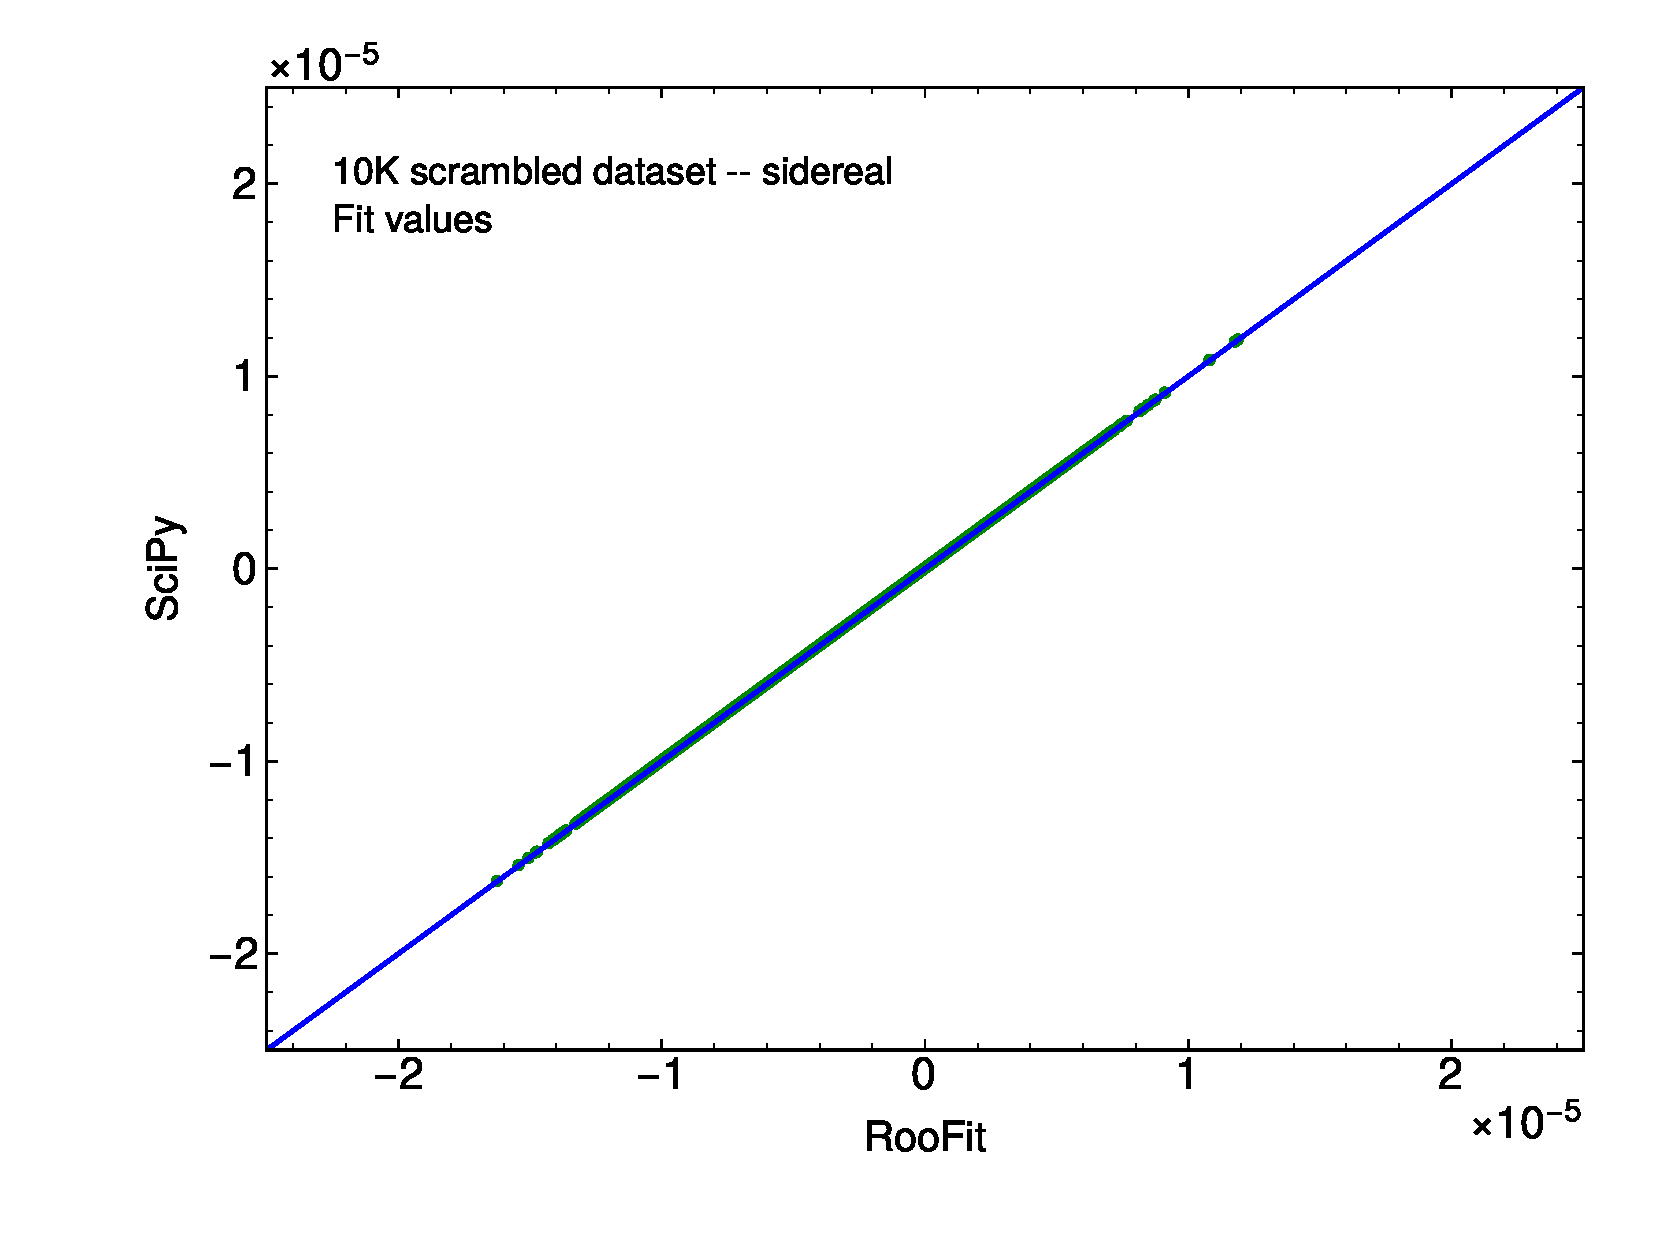
\includegraphics[width=0.45\textwidth]{figs/RooFit_SciPy/RooFit_SciPy_fit_results_2D_d[u,X,Z]}
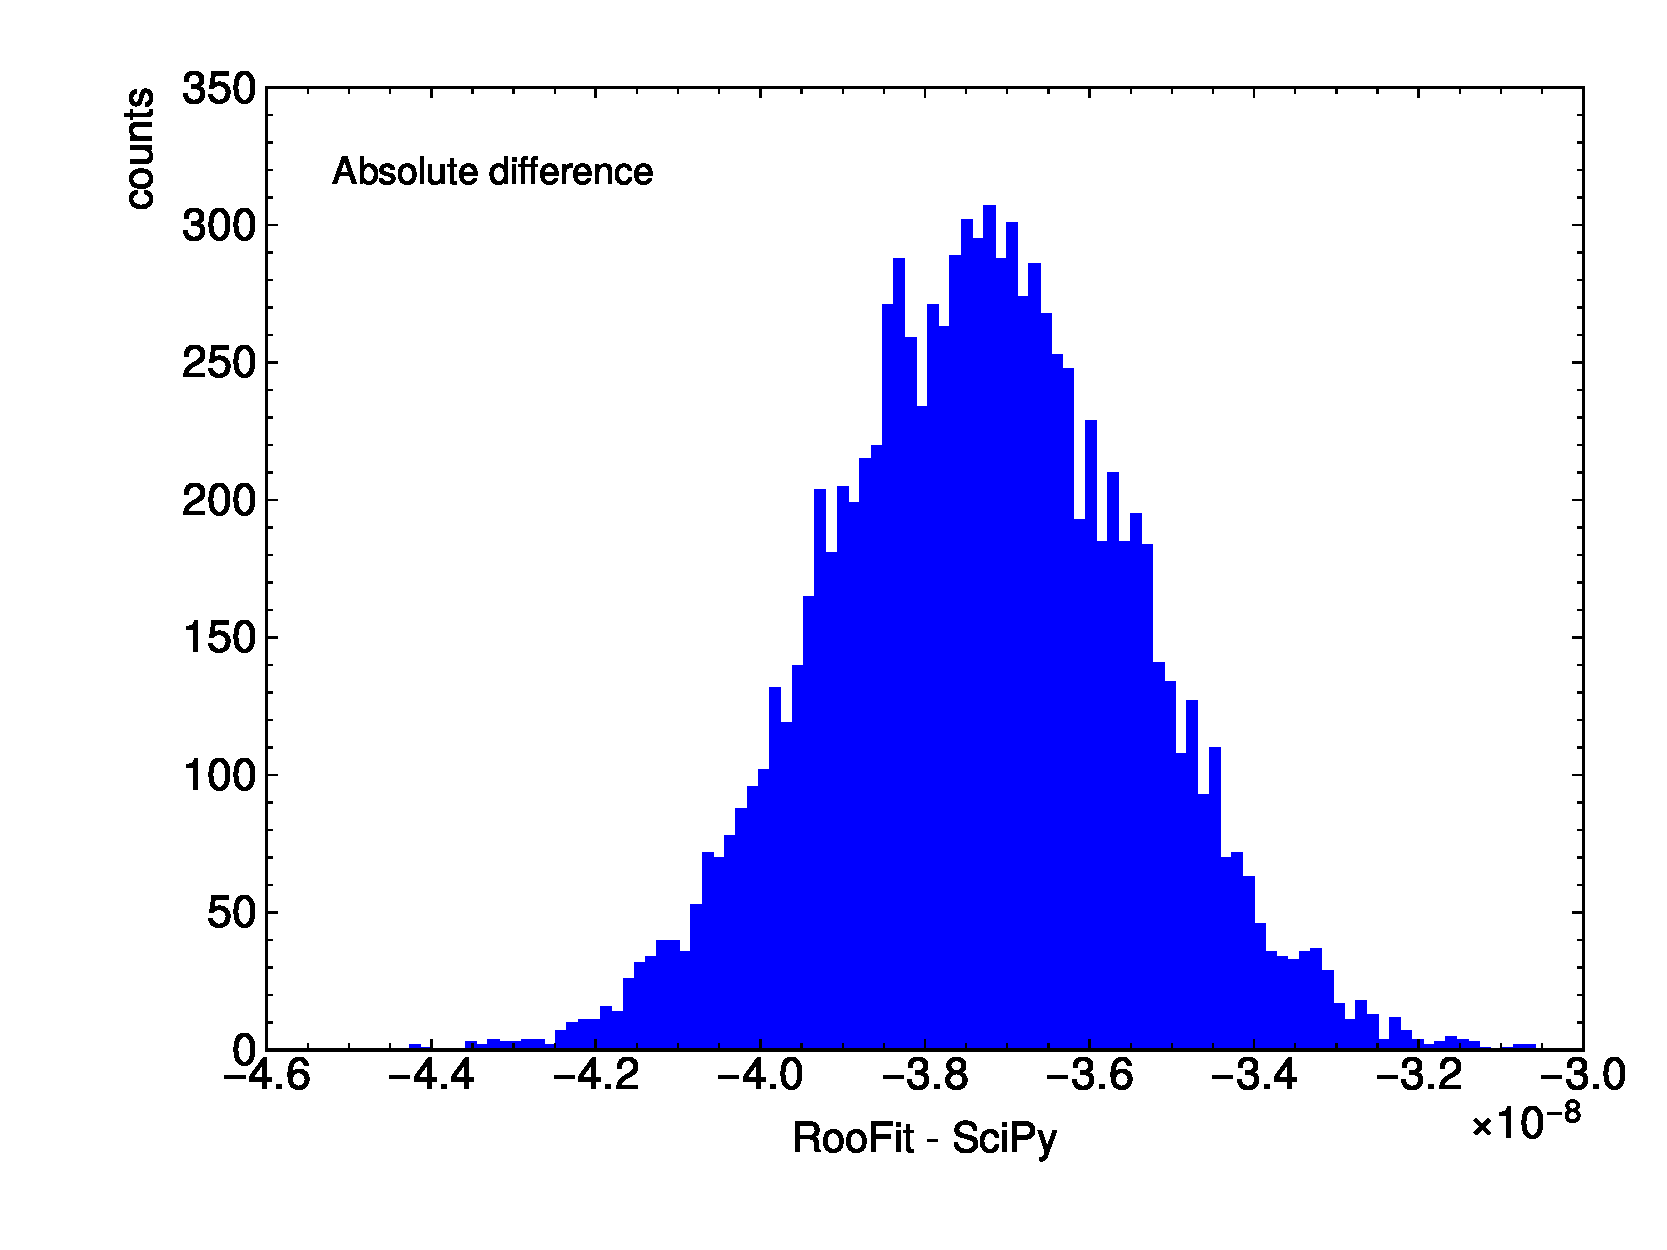
\includegraphics[width=0.45\textwidth]{figs/RooFit_SciPy/RooFit_SciPy_absolute_diff_d[u,X,Z]}\\

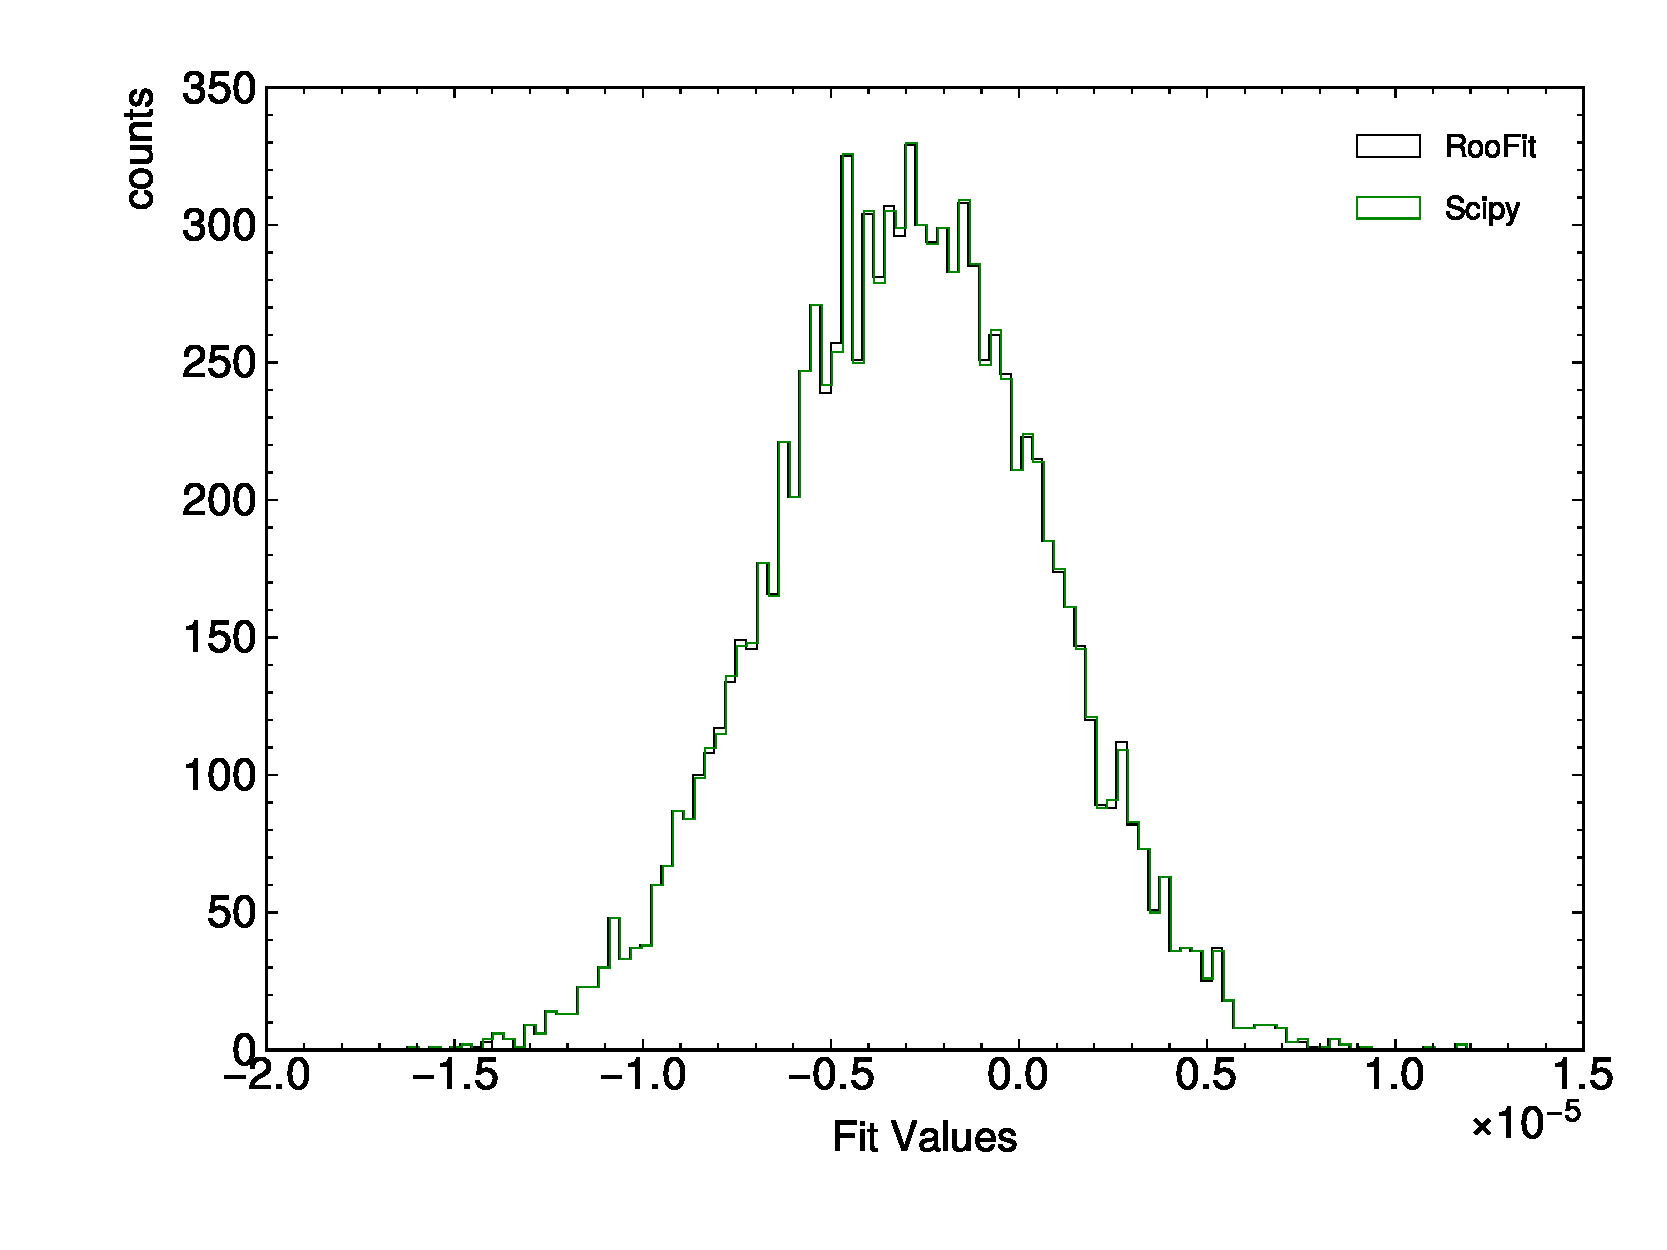
\includegraphics[width=0.45\textwidth]{figs/RooFit_SciPy/RooFit_SciPy_fit_results_hist_d[u,X,Z]}
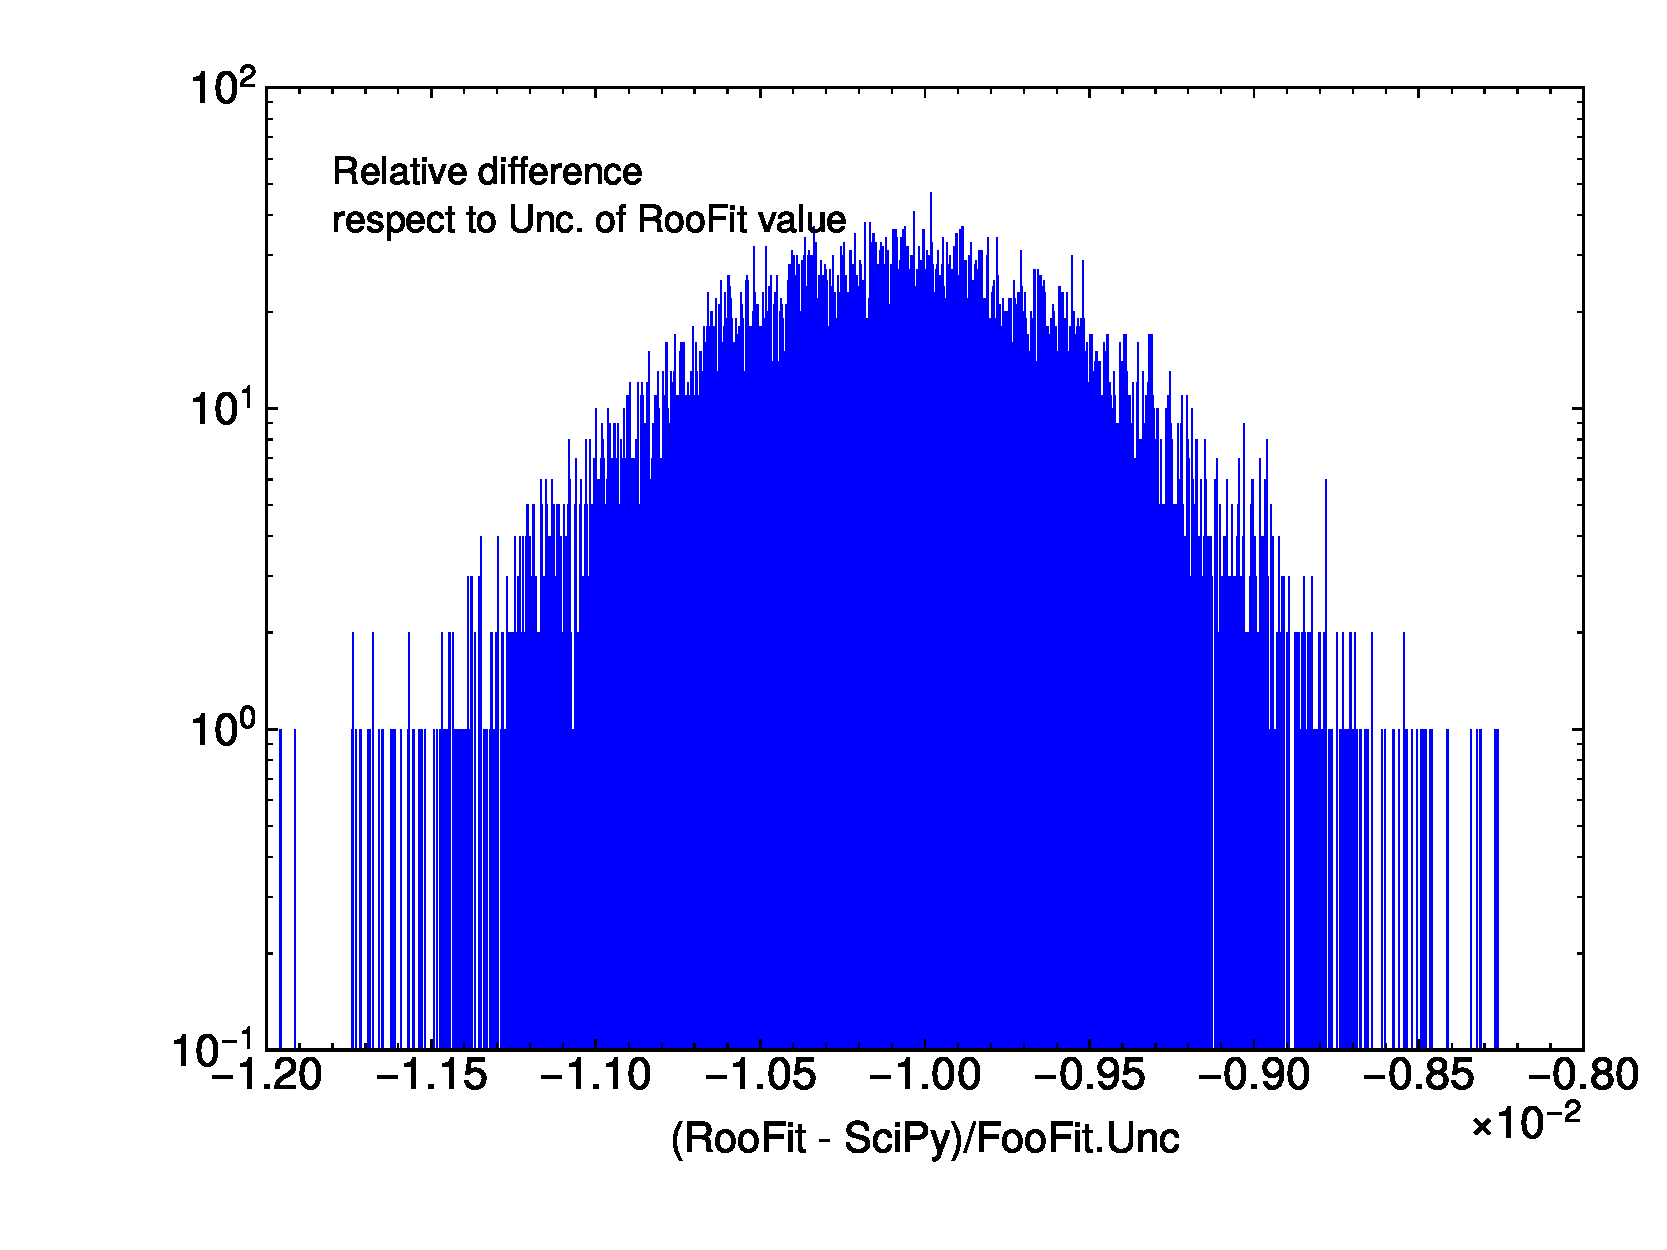
\includegraphics[width=0.45\textwidth]{figs/RooFit_SciPy/RooFit_SciPy_absolute_diff_significance_d[u,X,Z]}\\

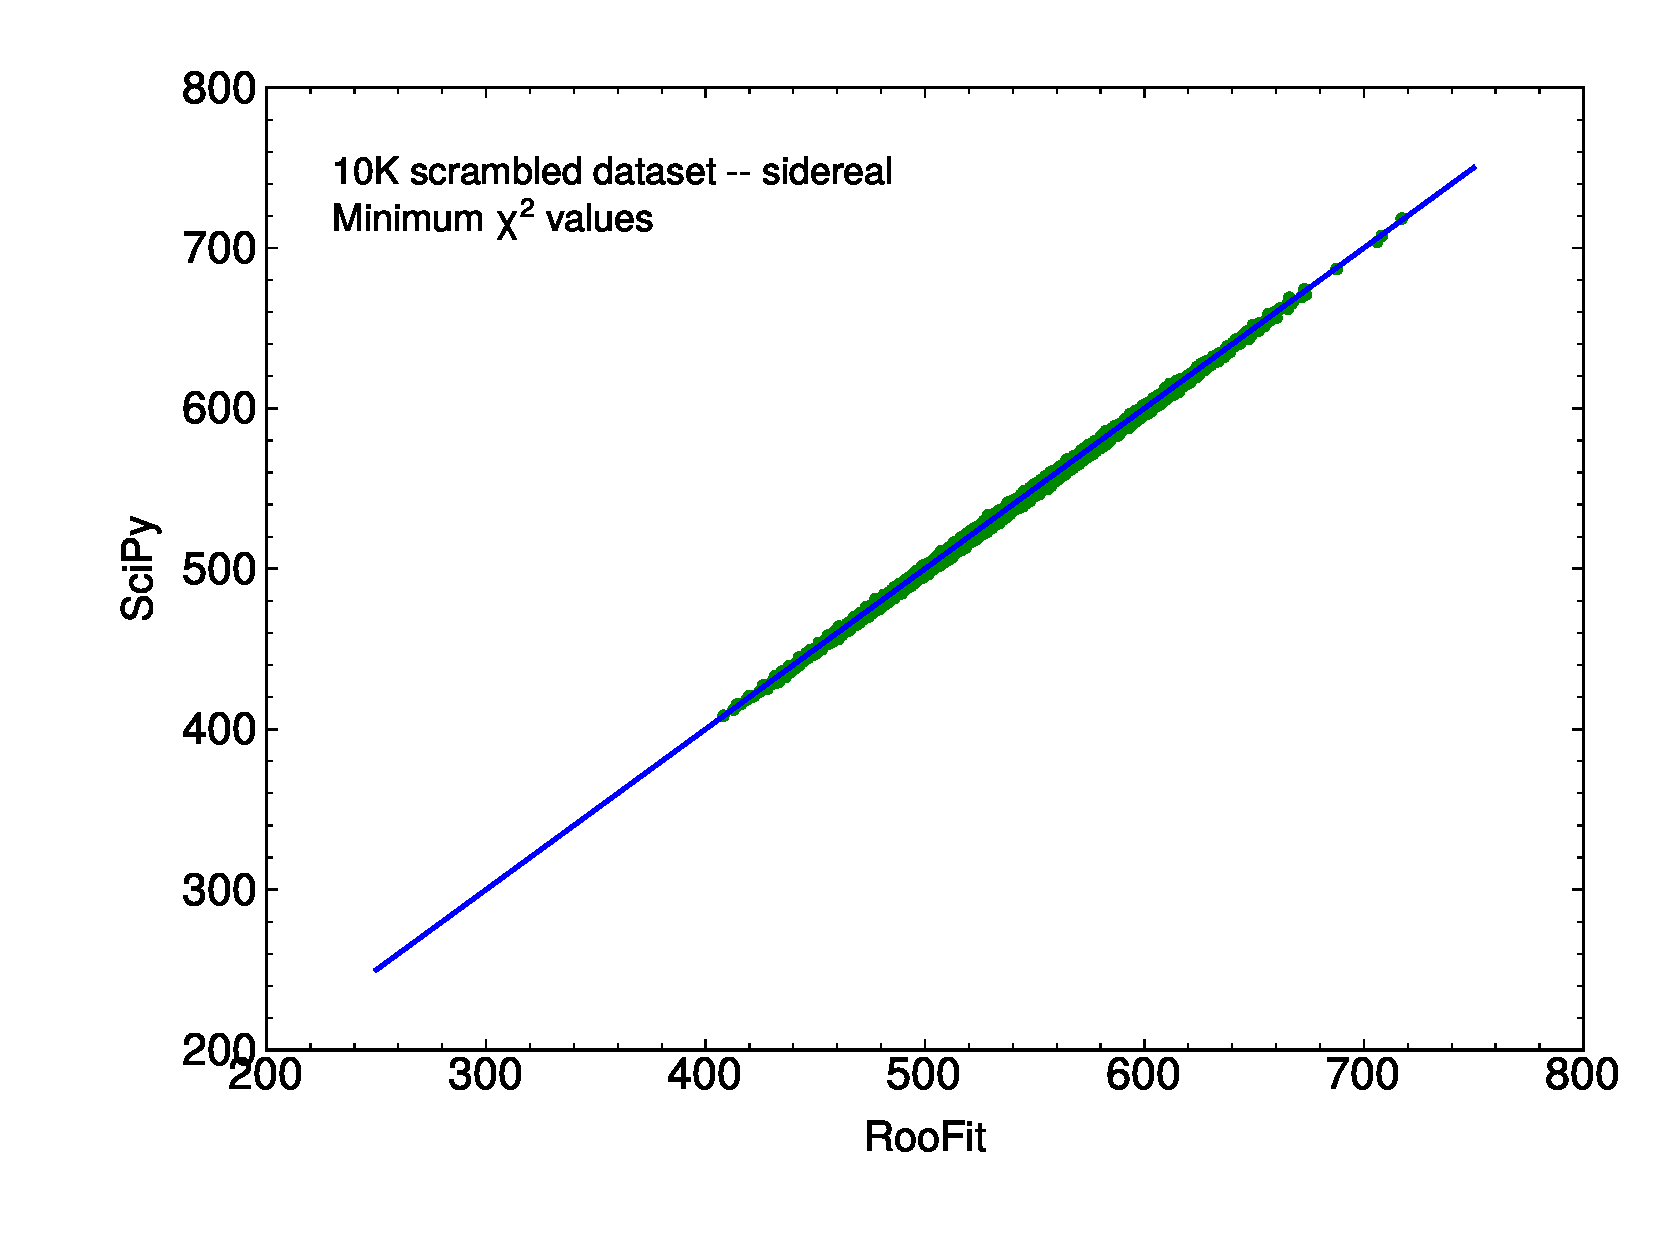
\includegraphics[width=0.45\textwidth]{figs/RooFit_SciPy/RooFit_SciPy_fit_results_2D_d[u,X,Z]_chi2}
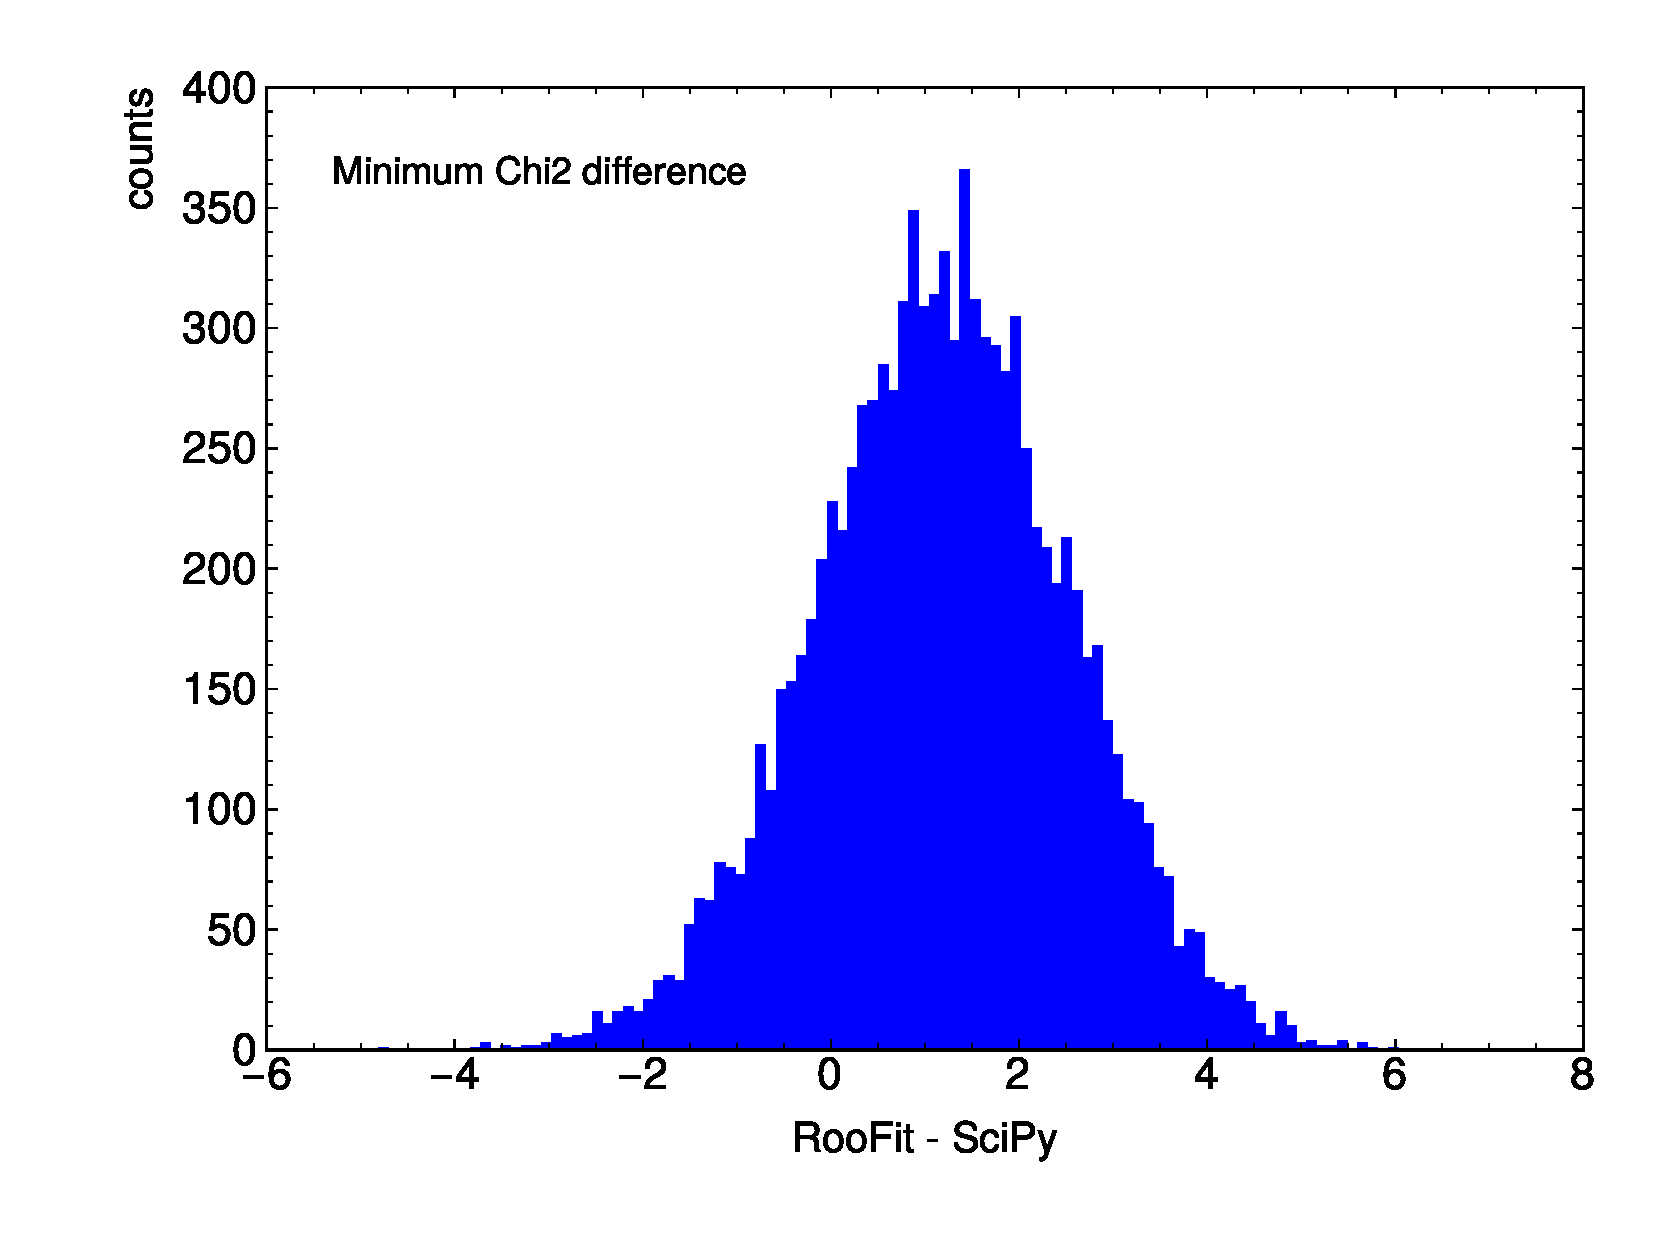
\includegraphics[width=0.45\textwidth]{figs/RooFit_SciPy/RooFit_SciPy_chi2_diff_d[u,X,Z]}\\

\caption{Comparison of the SME fit results from RooFit and SciPy on the 10K scrambled datasets. The top left plot shows the fit values; the x-axis is RooFit results, and the y-axis is SciPy results. The top right plot shows the difference between the RooFit and SciPy results. The middle left plot shows the distribution of the 10K fit results from RooFit and SciPy. The middle right plot shows the difference between RooFit and SciPy normalized to-fit errors from RooFit. The bottom left plot shows the minimum $\chi^{2}$ values from RooFit and SciPy fits. The bottom right plot shows the difference in minimum $\chi^{2}$.}
\label{fig:RooFit_SciPy_comparison_sme}
\end{figure}


%%%%
%% Generic
\begin{figure}[!ht]
\centering
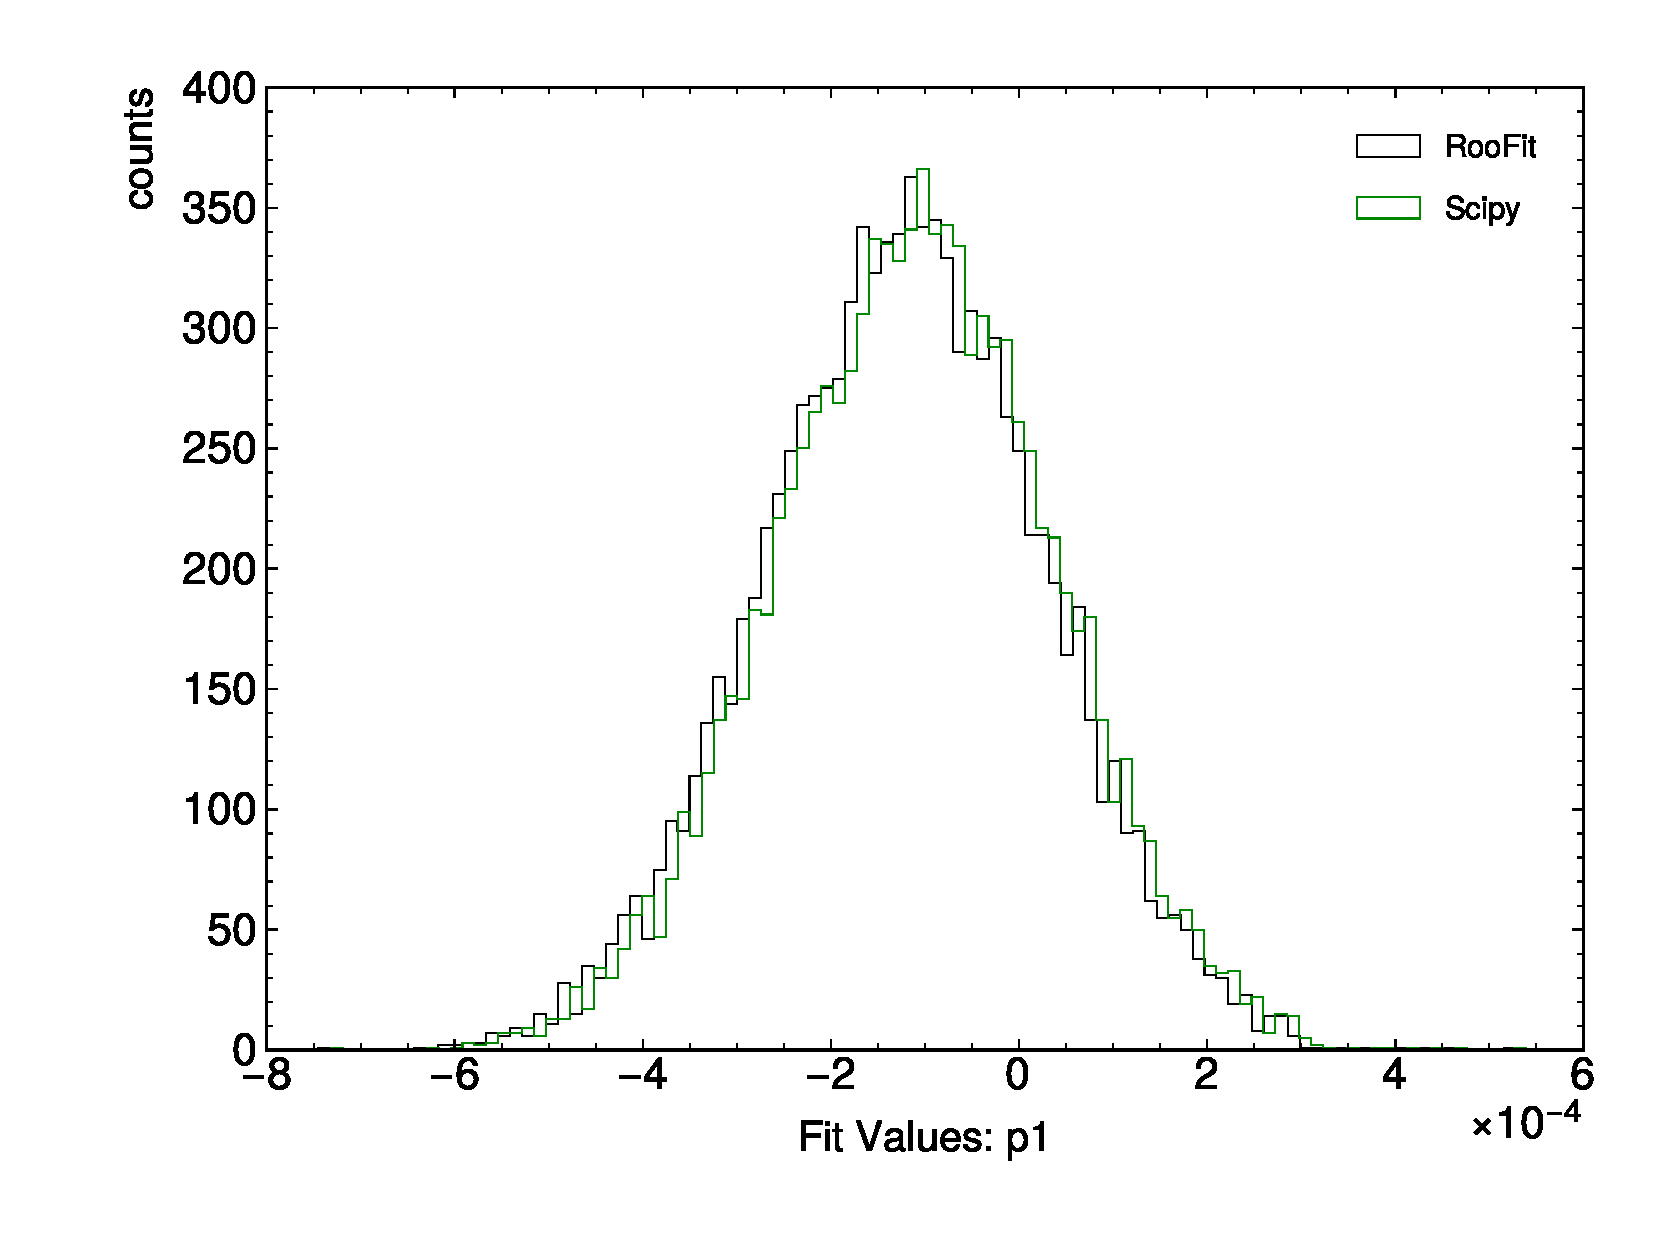
\includegraphics[width=0.45\textwidth]{figs/RooFit_SciPy/RooFit_SciPy_fit_results_hist_Sone_p1}
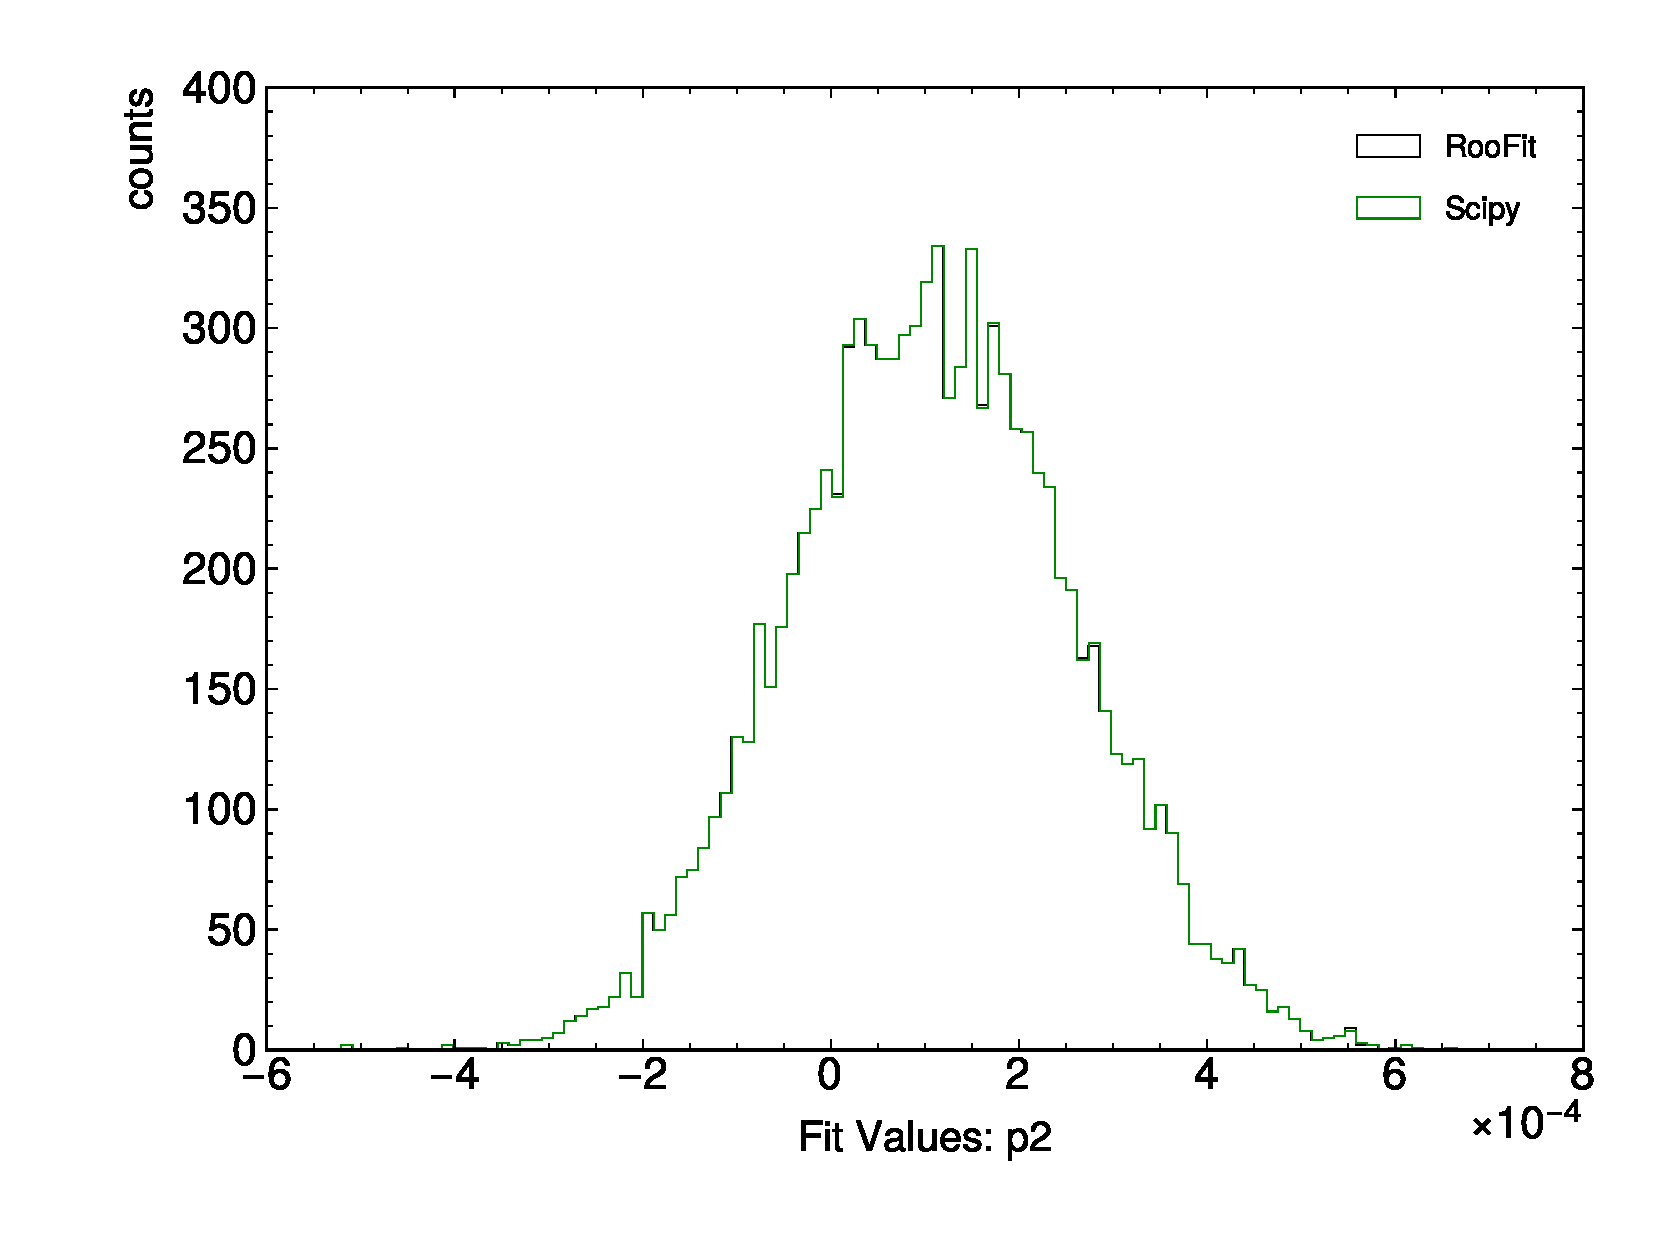
\includegraphics[width=0.45\textwidth]{figs/RooFit_SciPy/RooFit_SciPy_fit_results_hist_Sone_p2}\\

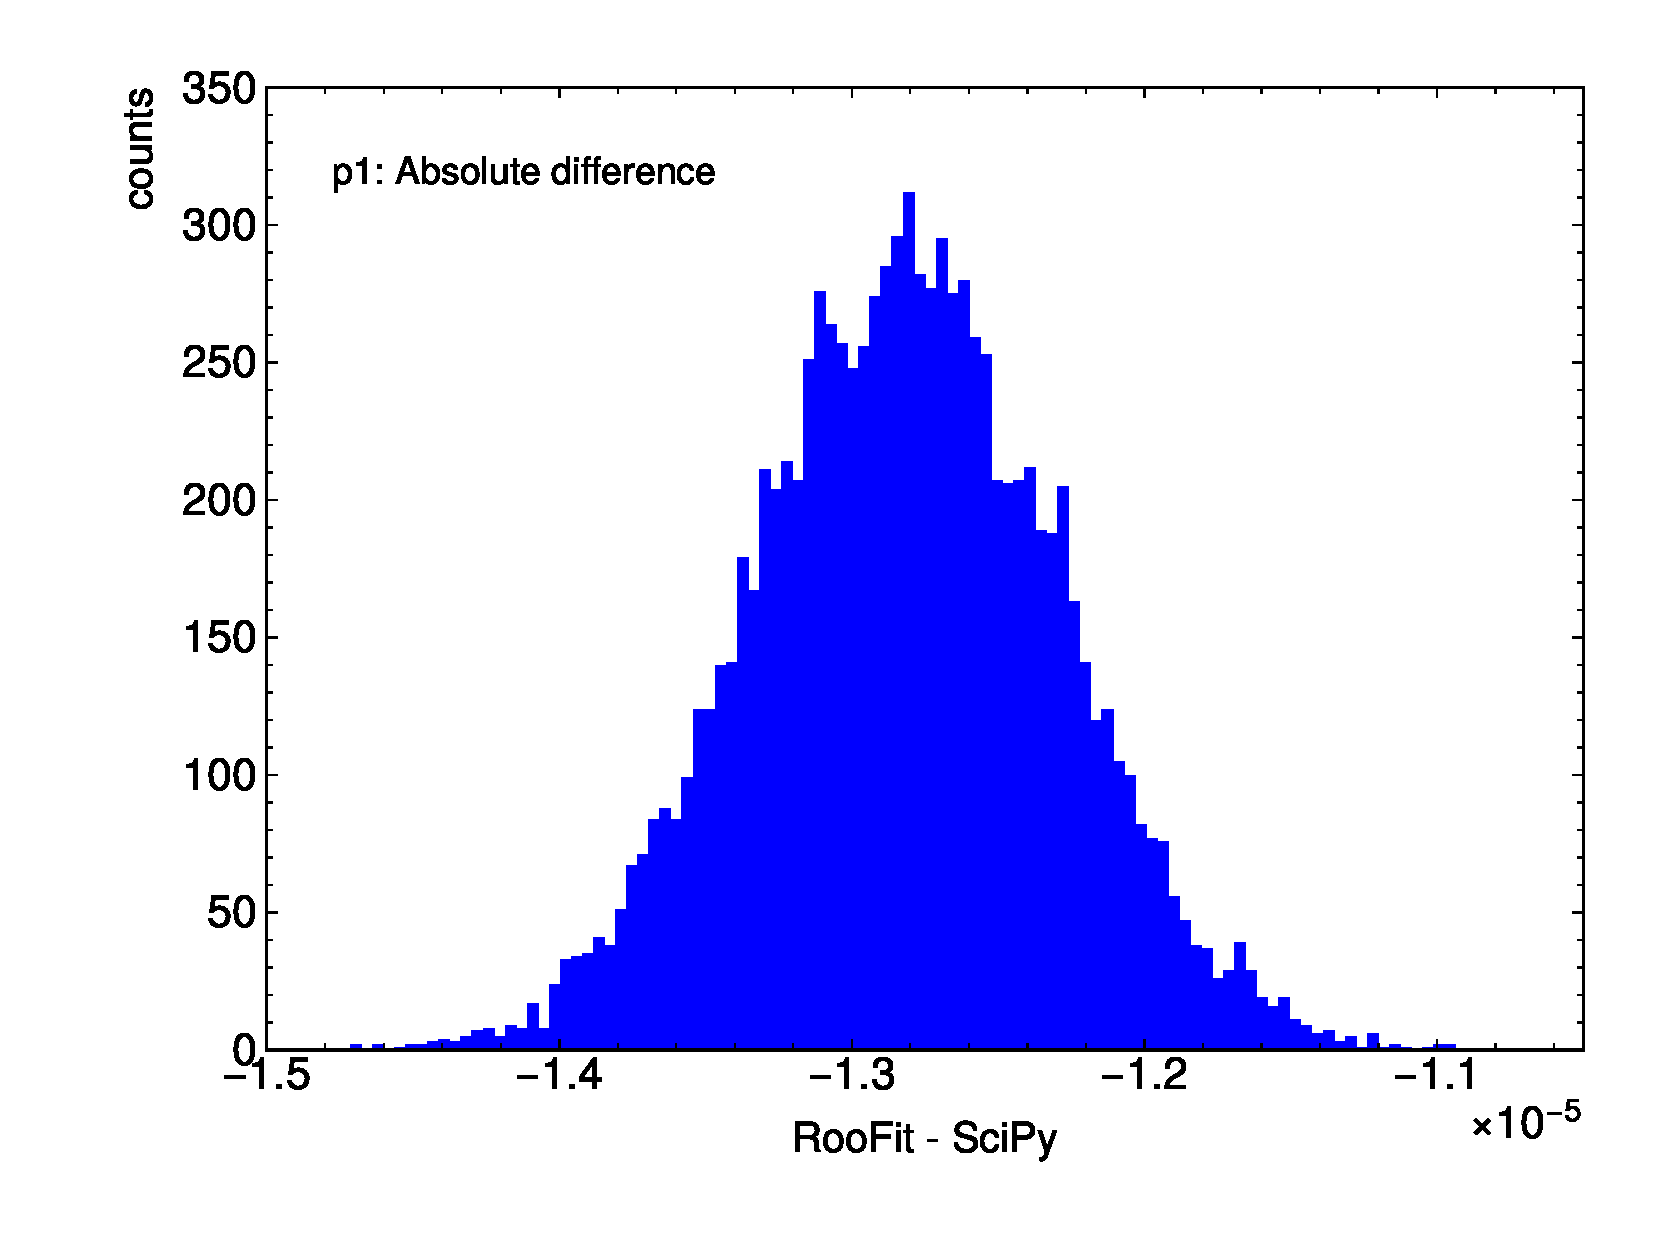
\includegraphics[width=0.45\textwidth]{figs/RooFit_SciPy/RooFit_SciPy_absolute_diff_Sone_p1}
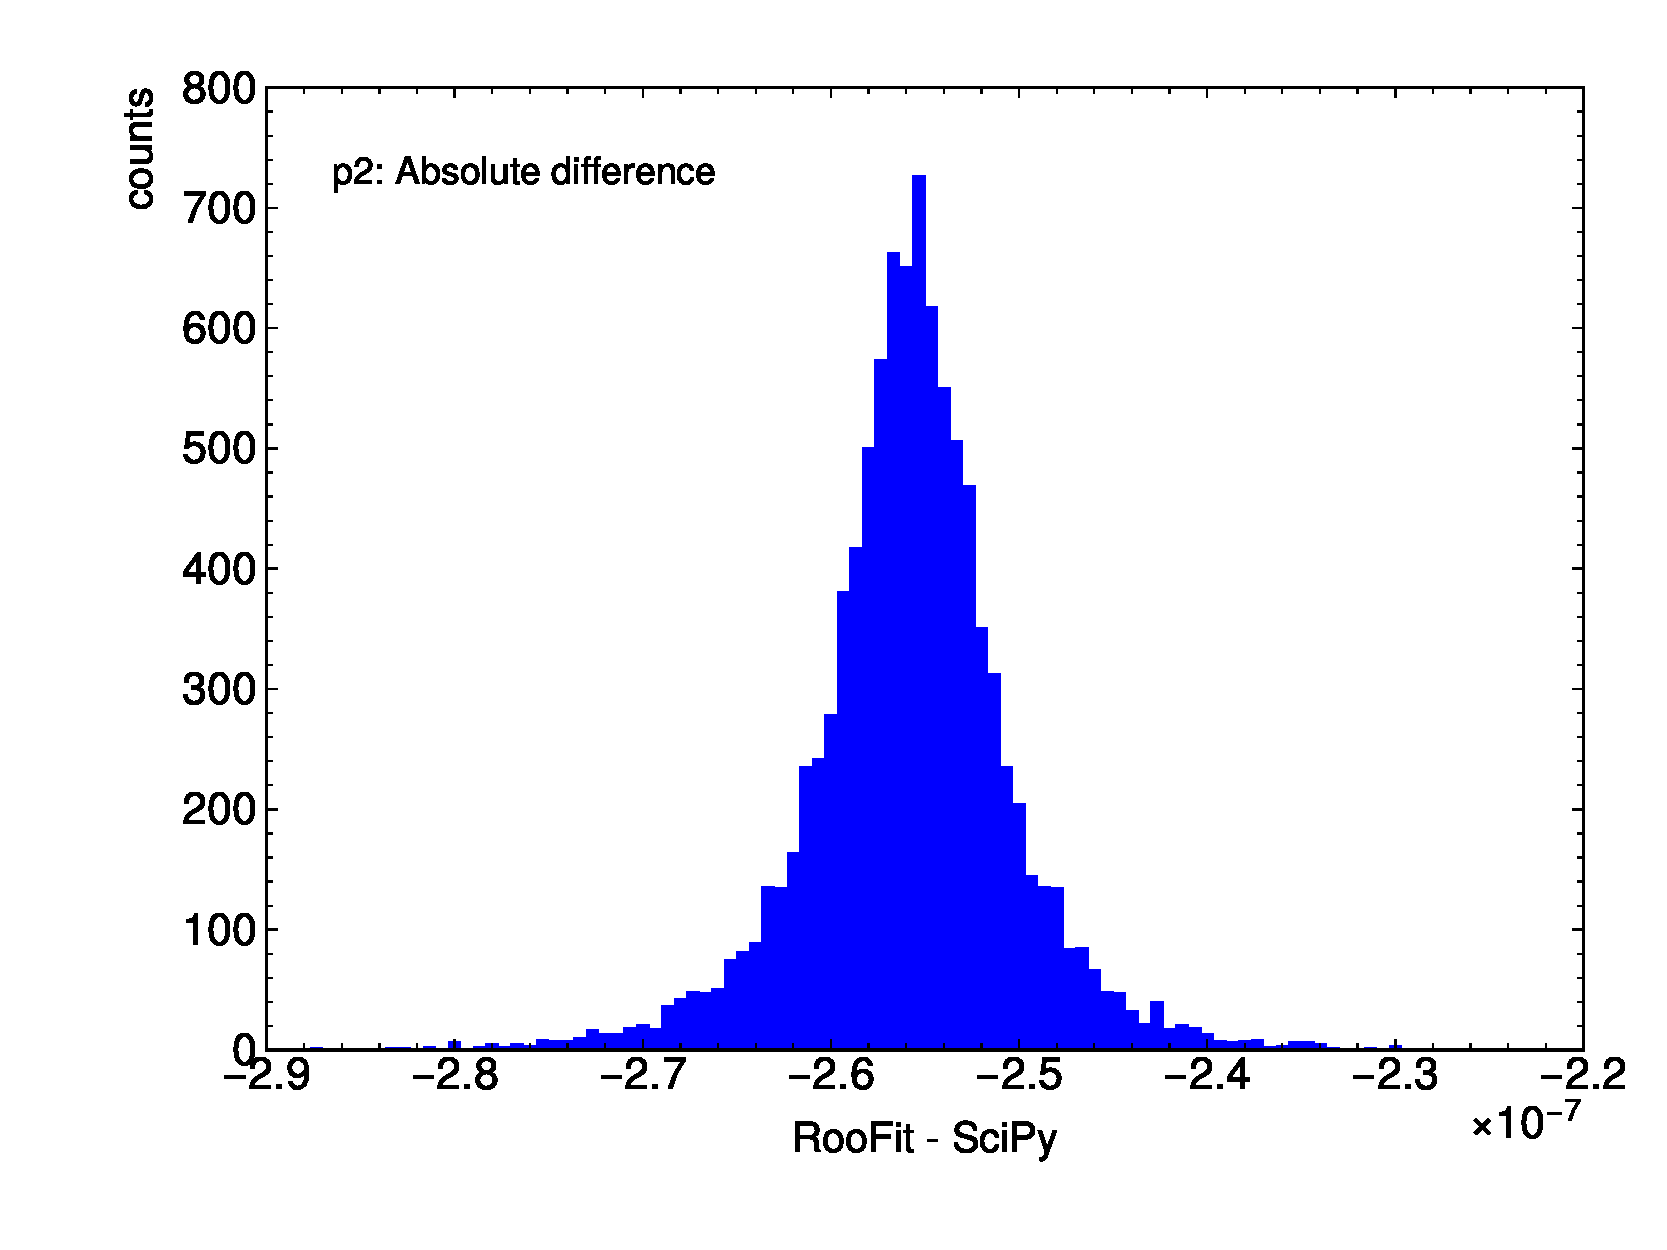
\includegraphics[width=0.45\textwidth]{figs/RooFit_SciPy/RooFit_SciPy_absolute_diff_Sone_p2}\\

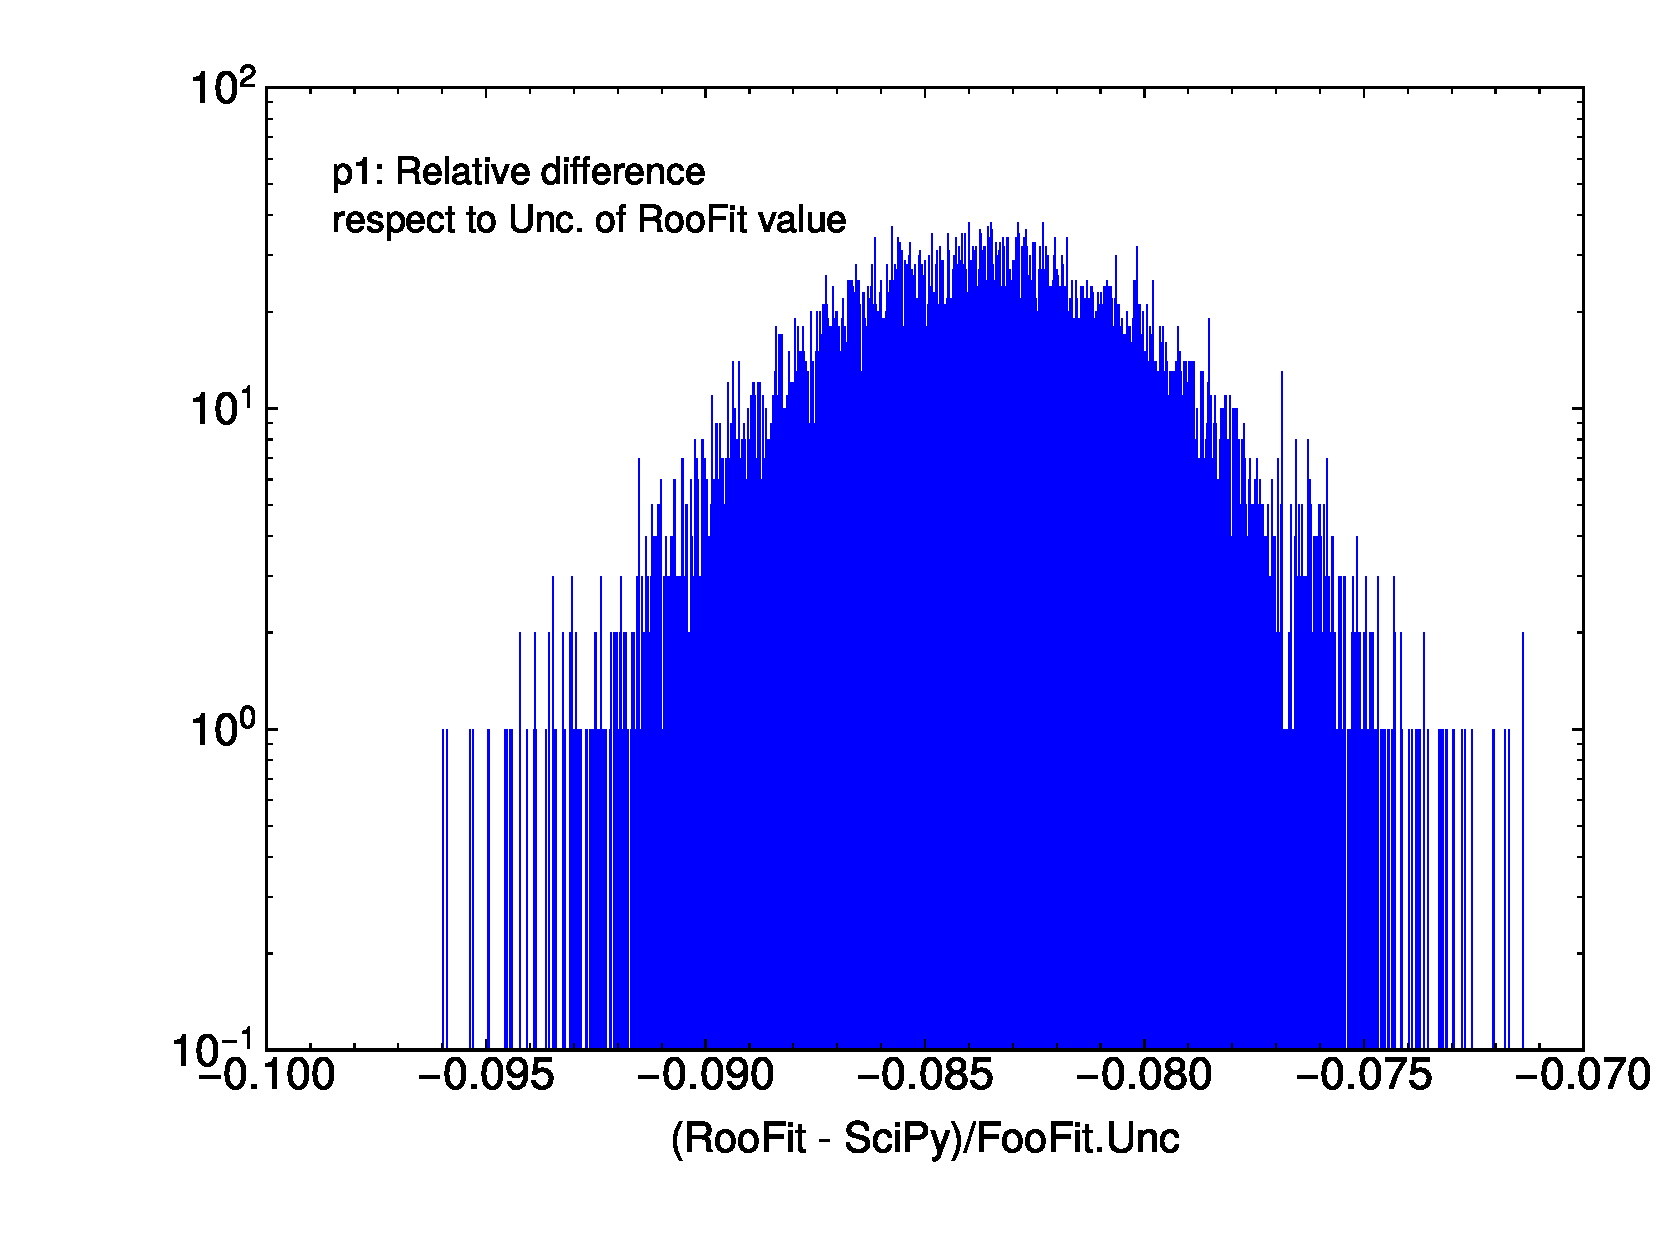
\includegraphics[width=0.45\textwidth]{figs/RooFit_SciPy/RooFit_SciPy_absolute_diff_significance_Sone_p1}
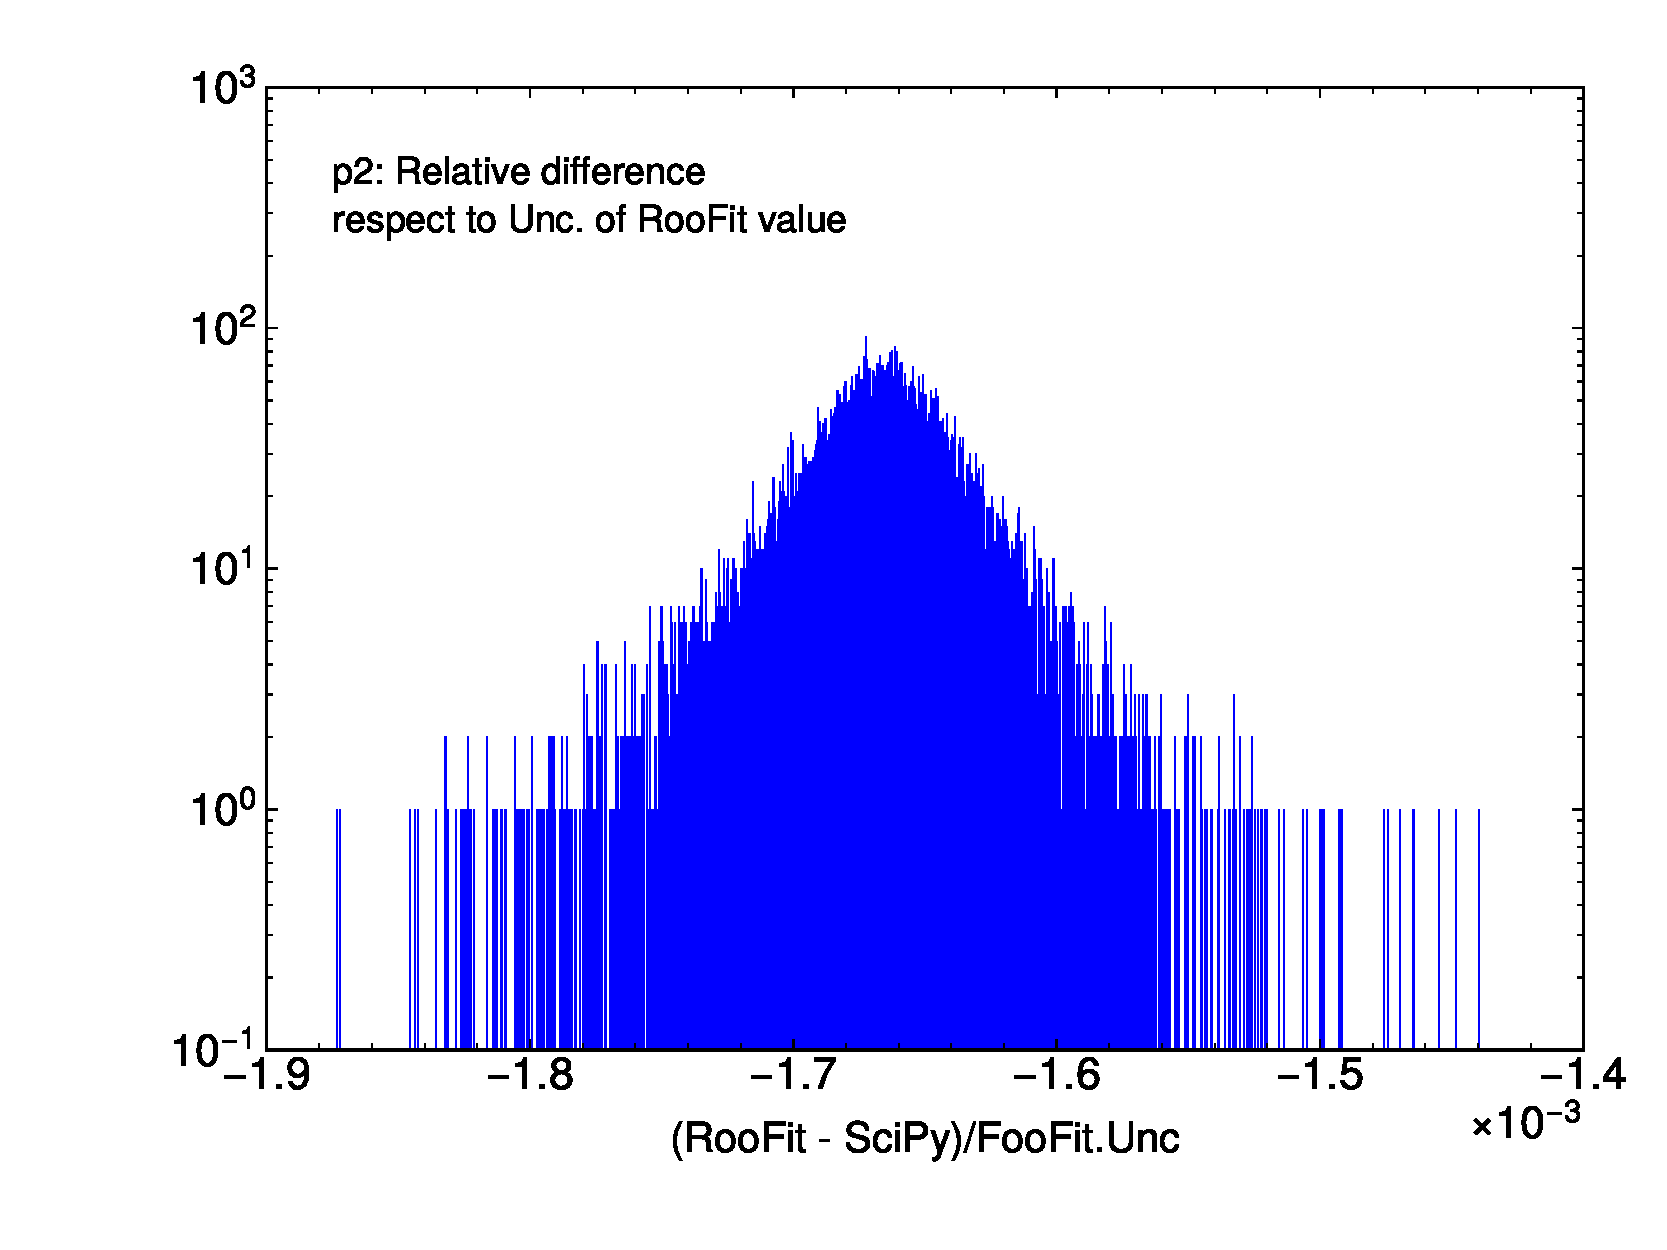
\includegraphics[width=0.45\textwidth]{figs/RooFit_SciPy/RooFit_SciPy_absolute_diff_significance_Sone_p2}\\

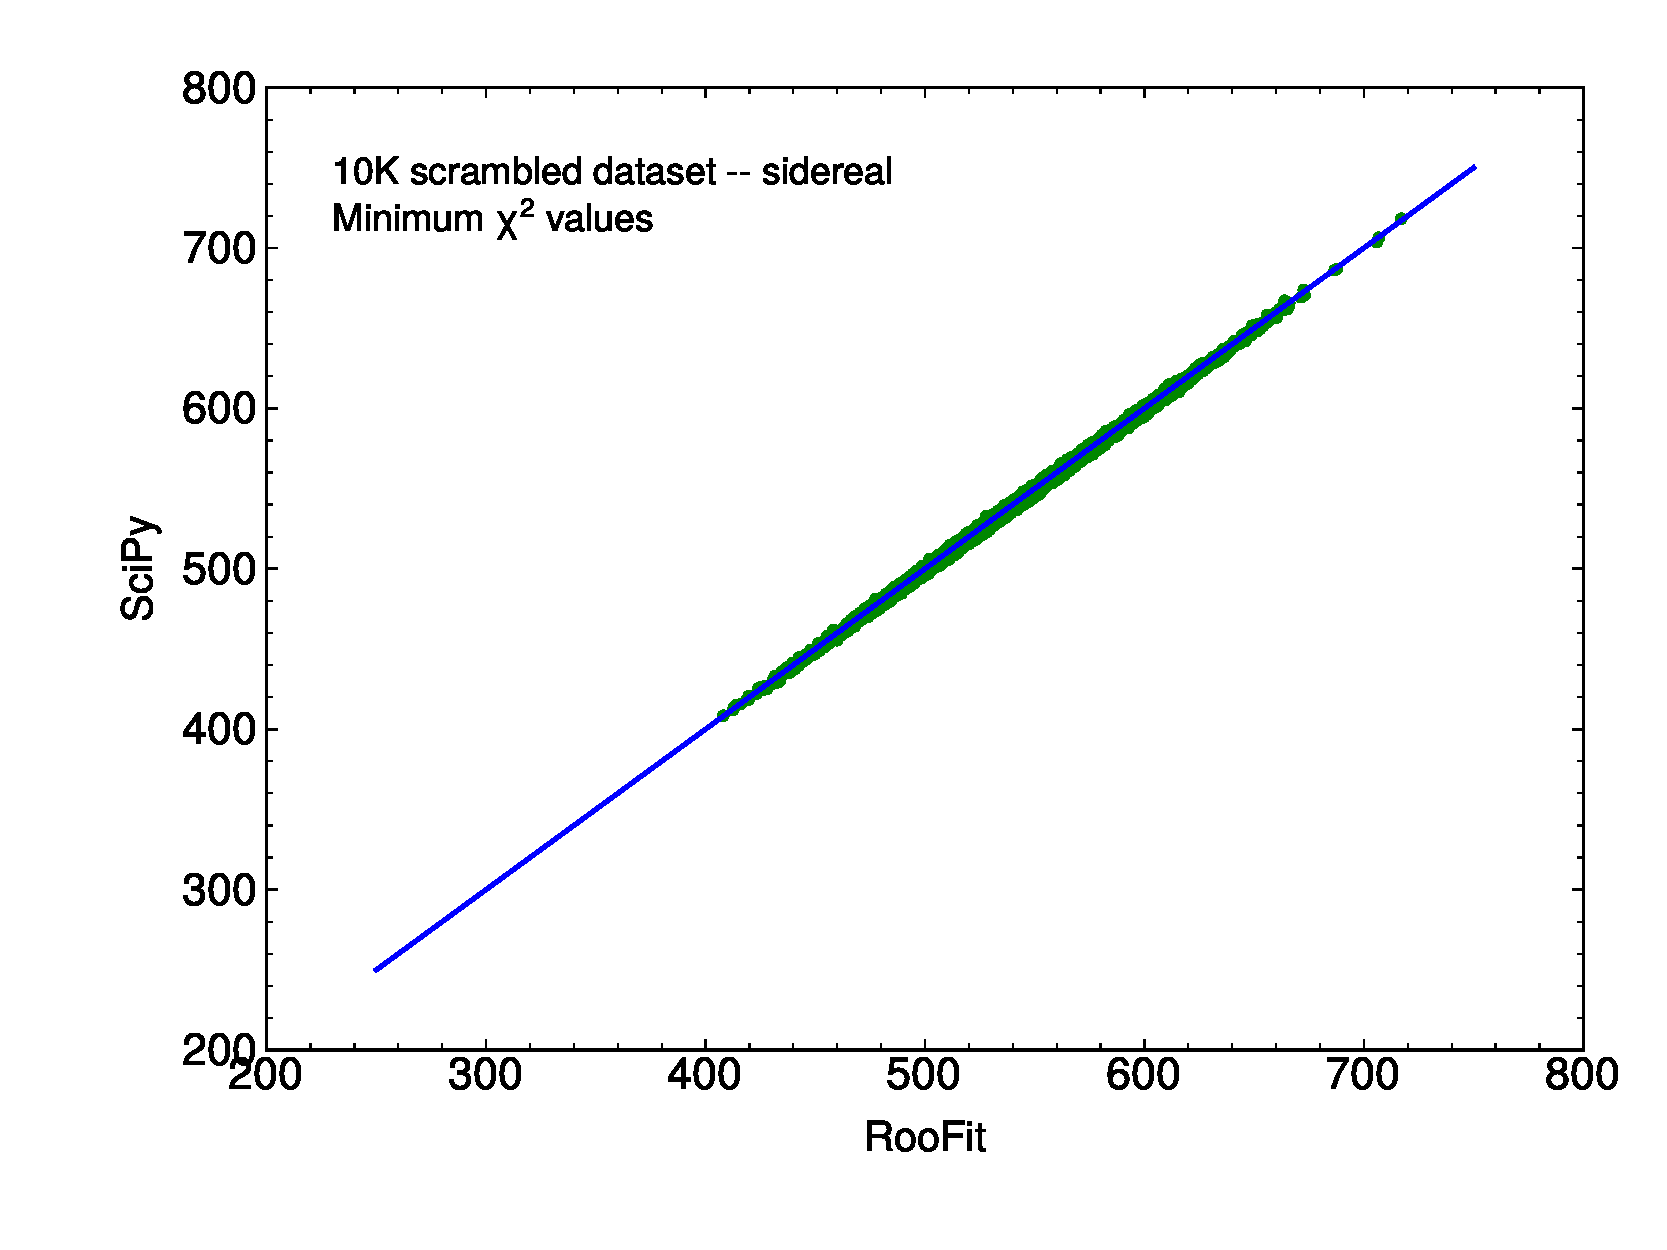
\includegraphics[width=0.45\textwidth]{figs/RooFit_SciPy/RooFit_SciPy_fit_results_2D_Sone_chi2}
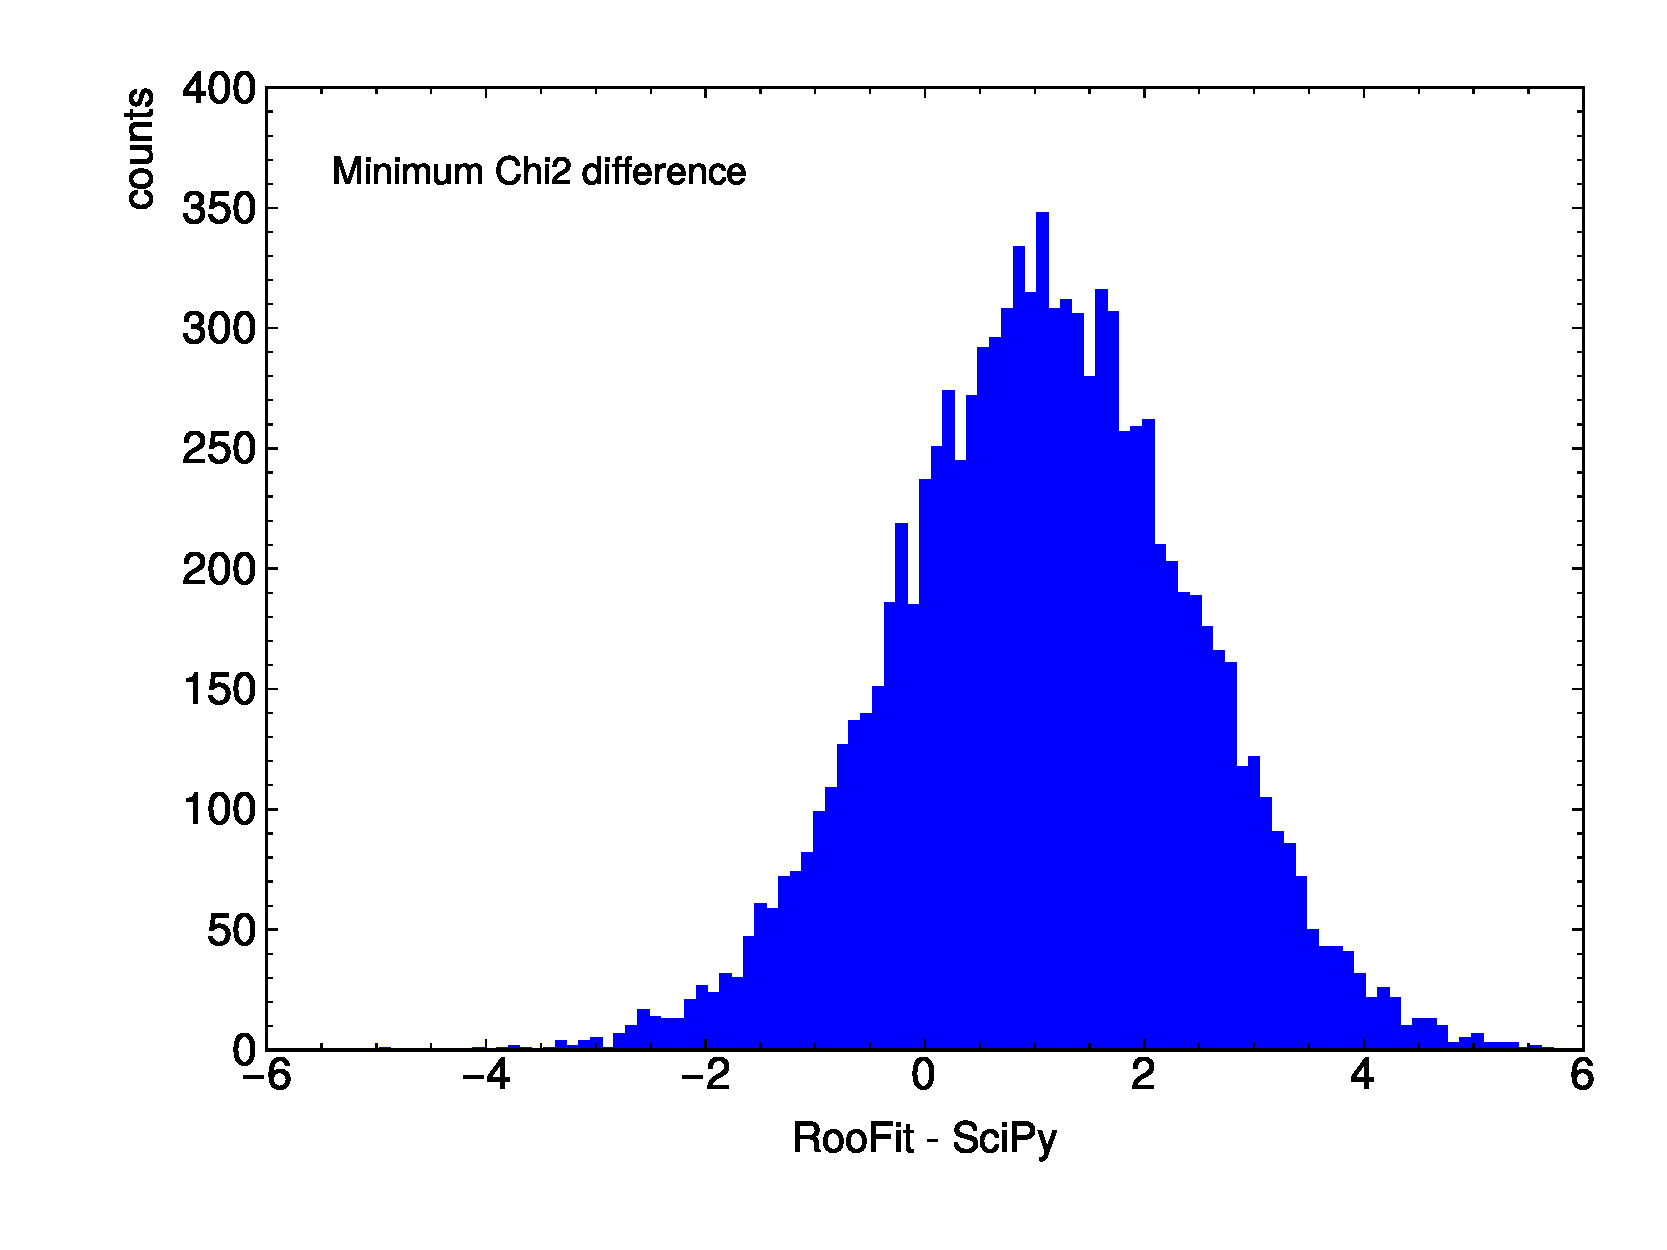
\includegraphics[width=0.45\textwidth]{figs/RooFit_SciPy/RooFit_SciPy_chi2_diff_Sone_chi2}\\

\caption{Comparison of the fit results of generic signals from RooFit and SciPy on the 10K scrambled datasets.
The top plots show the fit values of $p_{1}$ and $p_{2}$.
The plots in the second raw show the difference of the fit values from RooFit and SciPy fits. The plots in the third raw show the difference normalized to the fit errors from RooFit.
The bottom left plot show the minimum $\chi^{2}$ values from RooFit and SciPy fits; and the bottom right plot show the difference of the minimum $\chi^{2}$ values.}
\label{fig:RooFit_SciPy_comparison_generic}
\end{figure}